\section{Discretization}
\subsection{Introduction}
Real world data mining tasks involve discrete and continuous data. The algorithms able to handle continuous 
variables can impose some conditions previous to learning process. The violation of these conditions
produces a low classifier accuracy. On the other hand the learning process can require more CPU than for a 
corresponding task with discrete variables. Furthermore some datasets contain continuous 
and discrete variables adding an extra level of complexity to algorithms ~\cite{weiss91},
~\cite{catlett91b}, ~\cite{michalski78}.

A common method of dealing with this problem is to discretize continuous-value features, by 
breaking variable values into ranges. So an improvement of the discretization process could 
imply an improvement in classifiers accuracy. On the other hand discretization can be effective 
in a reduction in time to induce a classifier ~\cite{catlett91b}~\cite{dougherty95}~\cite{fayyad93}. 
Sometimes discretization can outperform some algorithms where some conditions related to algorithm about 
data distribution are violated.

A poor discretization algorithm can suppose an important lost in classifier accuracy. Furthermore 
depending on the classification algorithm, the same discretization policy will produce different classifier accuracies. 
Let's note that whilst Bayesian approaches for instance impose some conditions about data 
distributions, decision trees, on the other hand require sorting operations to deal with them, which 
increase learning times. In order to see the result of applying different discretization algorithms to 
induce different models an experiment was carried out ~\cite{dougherty95}. The conclusion is very 
clear: classifier accuracy depends on the discretization algorithm and on the model. However discretization 
is not an easy task because it has been shown that this is a NP-Complete problem 
with Naive-Bayes classifier, discretization is in general a NP problem: ~\cite{pazzani95},~\cite{elomaa03}. 

\subsection{Classes and Methods}
The class \verb=Discretization.java= implements some of the best known algorithms in the discretization
literature ~\cite{dougherty95}. On the other hand, another class: \verb=BlindDiscretization.java= 
has been built, allowing one to make a discretization based on a so called \emph{Discretization Policy}. 
This class, althought initially developed in order to test classical well known algorithms, has shown its utility
on other situations.

\subsubsection{Discretization.java}
Elvira allows one to perform a discretization of a two different form set of variables:
\begin{itemize}
	\item	Normal Discretization: each variable can be discretized by means of an algorithm and a different
			number of intervals.
	\item	Massive Discretization: all variables are discretized using the same algorithm and the same number
			of intervals.
\end{itemize}

In the following, we will explain the main methods to perform discretizations:
\begin{enumerate}
	\item	\verb=Discretization()=: it is the class constructor.
	\item	\verb=loadData(String Filename)=: method that allows one to load the database from a file.
	\item	\verb=setMode(int Mode)=: method that sets the way the discretization works; the possible values
			are:
			\begin{itemize}
				\item	NO\_DISCRETIZE: no discretization is made.
				\item	DISCRETIZE\_GLOBALLY: the discretization is performed globally.
				\item	DISCRETIZE\_INDIVIDUALLY: the discretization is made individually.
			\end{itemize}
	\item	\verb=setOperation(int Operation)=: method that allows to set operation mode, function of the previously
			selected mode.

			If the operation mode is set as \texttt{DISCRETIZE\_INDIVIDUALLY}, then the allowed operations are:
			\begin{itemize}
				\item	NORMAL\_OPERATION: discretizes each of the variables one by one.
				\item	MASSIVE\_OPERATION: all of the variables are discretized using the same parameters.
			\end{itemize}

			However, if the mode of operation is set as \texttt{DISCRETIZE\_GLOBALLY}, the only allowed operation is:
			\begin{itemize}
				\item	MASSIVE\_OPERATION.
			\end{itemize}
	\item	\verb=configureIndividual(int Method, int Intervals,Vector Options)=: method that configures the discretization
		 	for all variables if the mode is set as \texttt{MASSIVE\_OPERATION}.
			\begin{itemize}
				\item	\verb=Method=: method of discretization of use.
				\item	\verb=Intervals=: number of intervals to discretize.
				\item	\verb=Options=: discretization options of the algorithm.
			\end{itemize}
	\item	\verb=setGlobalOptions(Vector Options)=: method that allows to set additional options when the algorithm
			performs a massive discretization.
	\item	\verb=configureGlobal()=: method that configures the discretization, once it is set with 
			the \texttt{DISCRETIZE\_GLOBALLY} option.
	\item	\verb=apply()=: executes the configured discretization.
	\item	\verb=saveData(String Filename)=: method that allows one to save the discretized database in \verb=Filename=.
\end{enumerate}

\paragraph{Important Notes}
Performing discretization may lead to two non-controlled situations:
\begin{itemize}
	\item	Some missing values: in this case, the discretizer ignores these values and does not take
			them into account, so that the discretization algorithms never see them. This could lead to these
			values not being accounted for, nevertheless it is not important if one takes into account the
			nature of the algorithms.
	\item	Discretization of discrete values: if one detects that it exists a discrete variable to discretize,
			the variable's values are kept intact in the output file.
\end{itemize}

\begin{figure}
\label{cap08:02}
\begin{center}
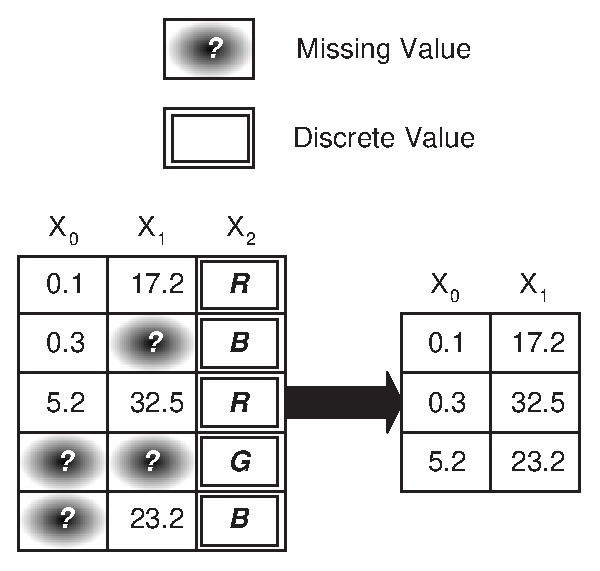
\includegraphics[width=45mm]{Learning/Preprocessing/fig/figure-8.02.ps} 
\end{center}
\caption{Missing Values and Discrete Variables}
\end{figure}

The consequences of these \emph{non-controlled} situations are:
\begin{itemize}
	\item	No algorithm has to be modified; implying that no further developments are needed.
	\item	The algorithms only take into account valid data in order to control the cutting points; in 
			some cases one could assume later on a lost of precision of the classifying methods. This is
			due to the fact that if we do not get enough representative data, the following discretizations
			are not the best ones.
\end{itemize}

This situation can be seen in figure 8.2.

\paragraph{Lexicographical Conventions}
From now on, and due to space constraints we will make the following assumptions:
\begin{itemize}
\item	\verb=java .../Discretization=
\item	\verb=java .../BlindDiscretizacion=
\end{itemize}
Where: \fbox{...} means  \verb=elvira/learning/preprocessing=
 
\subsubsection{BlindDiscretization.java}
In some situations, it may be suitable to do a discretization based on a predefined set of cut-points,
\verb=BlindDiscretization.java= allowing us to make this type of discretizations. In the following,
we will make some basic definitions:

Let's suppose that we have a database whith $M$ examples and each of them is labeled
with a class. This database can be denoted as $D=\{(x^{(w)},c^{(w)}), w=1,...,M\}$. 

A \emph{\textbf{discretization sequence}} for variable $X_{i}$ is denoted as $\lambda^{i}=<t_{1}^{i},\ldots,t_{k_{i}}^{i}>$ 
and it is an increasing sequence of real numbers.This means that the sequence verifies 
$t_{1}^{i}<t_{2}^{i}<\ldots<t_{k}^{i}$. Based on this definition a function for each variable is 
defined $f_{{\lambda}^{i}}: R \rightarrow  \{ 0,1,\ldots,k^{i} \}$ as:

\begin{equation}
f_{\lambda^{i}}(x_{i})=
	\begin{cases}
		0& \text{if }  x<t_{1}^{i} \\
		j& \text{if $t_{j}^{i} \leq x < t_{j+1}^{i}$ $j=1,\ldots,k-1$}\\
		k& \text{if } x \geq t_{k}^{i} 
	\end{cases}
\end{equation}

A \emph{\textbf{discretization policy}} $\Lambda$ is defined as a set of $n$ discretization sequences, each of them
is originally related to each continuous variable.  By the application of 
$\Lambda=<\lambda_{1},\ldots,\lambda_{n}>$ means that if we apply this discretization 
policy to a database $D$, a new \emph{discretized} database will be obtained. This new database is 
denoted as $D^{d}=\{(\mathbf{x}^{(w)d},c^{(w)}), w=1,...,N\}$, verifying that $\Lambda(D)=D^{d}$. Note that 
class label remains invariable.
	
To be able to make this task, the class requires the specification of three files:
(see figure 8.3):
\begin{itemize}
	\item	Fichero 1 - Name of the file with the continuous database.
	\item	Fichero 2 - Name of the file with the discretized database.
	\item	Fichero 3 - Name of the file with discretization policy.
\end{itemize}

\begin{figure}
\label{cap08:03}
\begin{center}
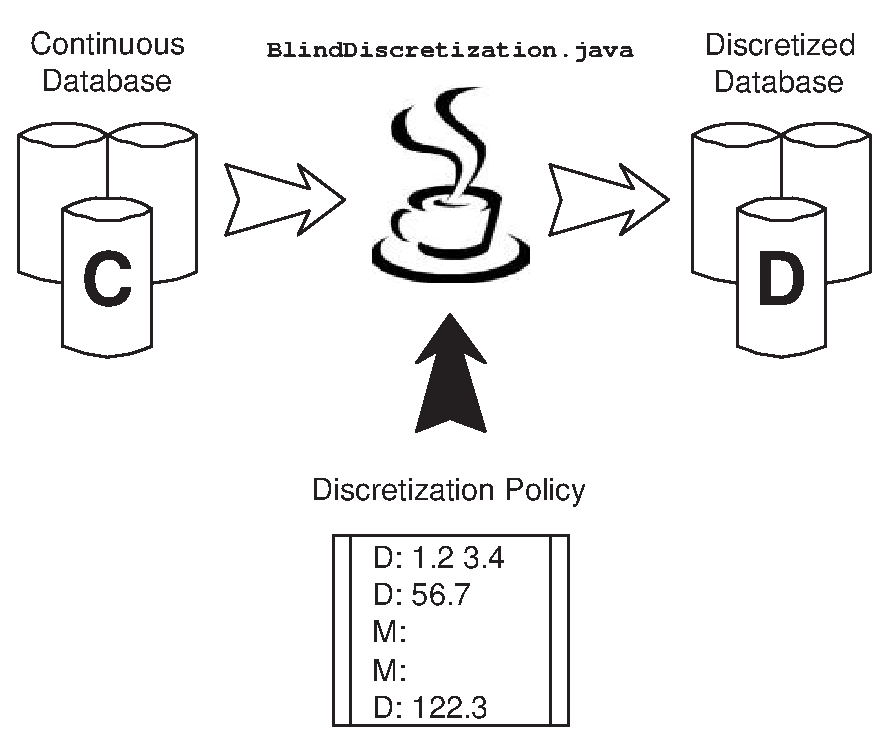
\includegraphics[width=90mm]{Learning/Preprocessing/fig/figure-8.03.ps} 
\end{center}
\caption{Policy based Discretization}
\end{figure}

Thus, it will be necessary to explain the discretization policy file format.

\paragraph{Policy File format}
It has to be an ASCII file. We can thus create a policy file with a simple editor (e.g. Notepad,
in windows, vi, emacs or other in UNIX, but never using applications that modify the
file structure, e.g. Word, Wordperfect, ...).

The file format is the one specified in figure 8.4

\begin{figure}
\label{cap08:04}
\begin{center}
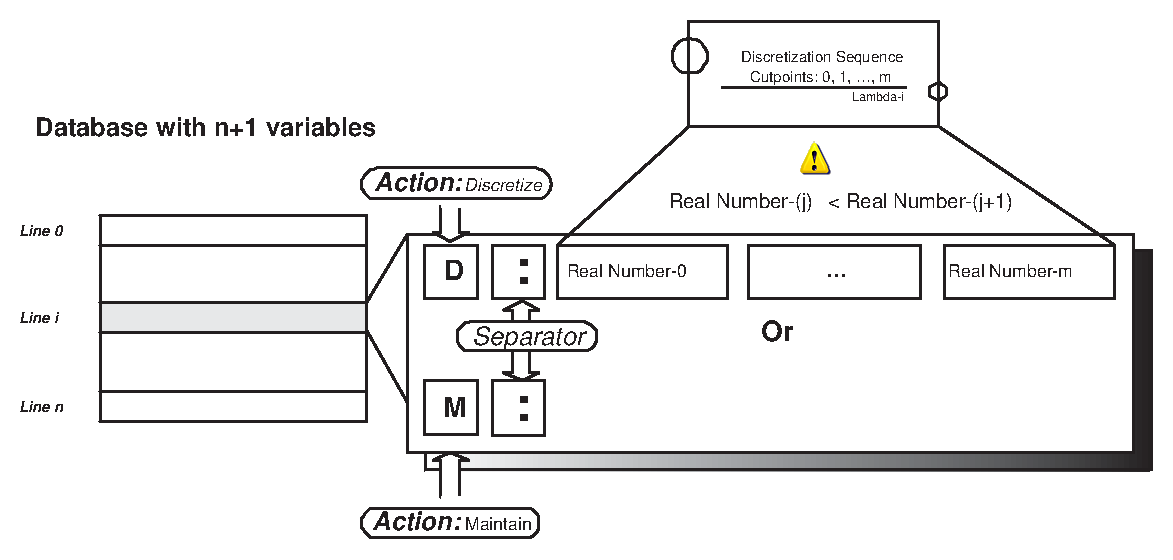
\includegraphics[width=130mm]{Learning/Preprocessing/fig/figure-8.04.eps} 
\end{center}
\caption{Policy File Format}
\end{figure}

The mathematical interpretation of the discretization policy file can be better understood in figure 8.5

\begin{figure}
\begin{center}
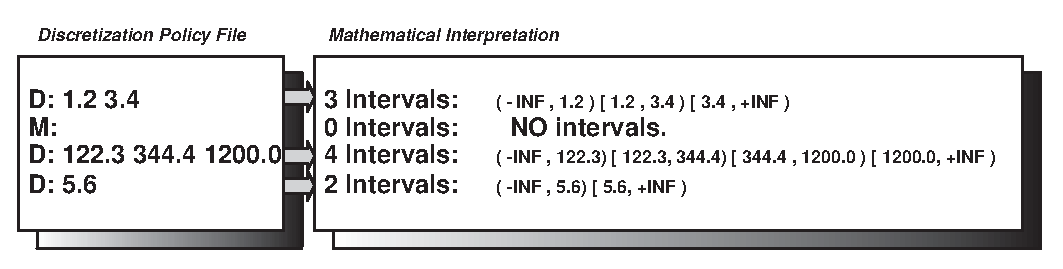
\includegraphics[width=130mm]{Learning/Preprocessing/fig/figure-8.05.eps} 
\end{center}
\label{cap08:05}
\caption{Mathematical Interpretation}
\end{figure}


To make things clearer, we will explain it with an example.

\paragraph{Example of creation of a policy file}
Let's assume that we have a 5 variables and a class. The characteristics of these variables are:
\begin{itemize}
	\item	Variable 1: Values belong to the interval [1000,2000].
	\item	Variable 2: Values observed are in the interval [-90,50]
	\item	Variable 3: Its values are: VERDE, y ROJO.
	\item	Variable 4: Values observed are in the interval [10.0,12.5]
	\item	Variable 5: Its values are: FRIO, CALIENTE y TEMPLADO.
	\item	Variable Clase: It has the values: ALTO, MEDIO y BAJO.
\end{itemize}

Let's supose  that we would like to apply the following discretization policy:
\begin{itemize}
	\item	Variable 1: It is not discretized.
	\item	Variable 2: It is discretized in 2 intervals and the cut-point is: 5.0.
	\item	Variable 3: Tt is not discretized.
	\item	Variable 4: It is discretized in 3 intervals. The cut-points are: 11.0 y 11.5.
	\item	Variable 5: It is not discretized.
\end{itemize}


The corresponding policy file will be \verb=myPolicy.dat=:

\begin{lstlisting}[frame=trBL, caption=myPolicy.dat, label=PolicyEx]{}
M:
D: 5.0
M:
D: 11.0 11.5
M:
M:
\end{lstlisting}

Now, we will proceed to the discretization based on the previously defined policy:

\begin{lstlisting}[frame=trBL, caption=Running Example, label=PolicyRunEx]{}
$ java .../BlindDiscretization myDATA.dbc myDATA-Disc.dbc myPolicy.dat
Discretizing and Reporting ...
Blind Discretization...Ok.
$
\end{lstlisting}

Next, we will describe a discretization a more detailed example based on policies:
\begin{enumerate}
	\item	\verb=BlindDiscretization()=: it is the class constructor.
	\item	\verb=loadDiscretization(String Filename)=: It is the method that allows to read
			the policy file.
	\item	\verb=discretize(String InputFilename, String OutputFilename)=: It is the method that executes
			the discretization.
		\begin{itemize}
			\item	\verb=InputFilename=: It is the name of the input file to discretize.
			\item	\verb=OutputFilename=: It is the name of the discretized file.
		\end{itemize}
\end{enumerate}

\subsection{Use-Case Specifications}
There exist two work possibilities with the discretization:
\begin{itemize}
	\item	Command-Line Interface (CLI): we can only make massive discretizations with the va\-ria\-bles.
	\item	Graphical-User Interface (GUI): Not only can we make massive discretizations with the variables,
			but also personalized discretization for each variable, i.e. we can choose for each variable
			the algorithm and number of intervals.
\end{itemize}

Even more, if we use the \verb=Discretization.java= API.

In the following table we can resume the differences between different interfaces:
\begin{table}[hbt]
\begin{center}
\begin{minipage}[b]{5cm}
\begin{tabular}{|l|c|c|c|}
	\hline
				   &    CLI	&	GUI	&	API	\\
	\hline
	\hline
	It allows automatization	   &	YES	&	NO	&	YES	\\
	\hline
	Collective Discretization   &	YES	&	YES	&	YES	\\
	\hline
	Individual Discretization  &	NO	&	YES	&	YES	\\
	\hline
\end{tabular}
\end{minipage}
\end{center}
\caption{Differences between CLI, GUI and API}
\label{cap08:tab01}
\end{table}

\subsubsection{Command-Line Interface}
The usage of the discretization using \verb=CLI= can be obtained executing the following:

\begin{lstlisting}[frame=trBL, caption=CLI Help, label=CLIHelp]{}
$ java .../Discretization
USAGE: <program> <input file.dbc> <output file.dbc> <algorithm> 
<intervals> <options>

<algorith> :
Algorith: 0 => EQUAL FREQUENCY
Algorith: 1 => EQUAL WIDTH
Algorith: 2 => SUM SQUARE DIFFERENCES
Algorith: 3 => UNSUPERVISED MONOTHETIC CONTRAST
Algorith: 4 => K MEANS

<intervals> :
Integer > 1

<options>   :
Only with Sum Square Differences: Real > 0
$
\end{lstlisting}

As it can be observed, we can not only make massive discretization and global operations.

\subsubsection{Graphical-User Interface}	
The step before we make any discretization is to load database-cases file, as seen in figure 8.6

\begin{figure}[htb]
\begin{center}
\label{cap08:06}
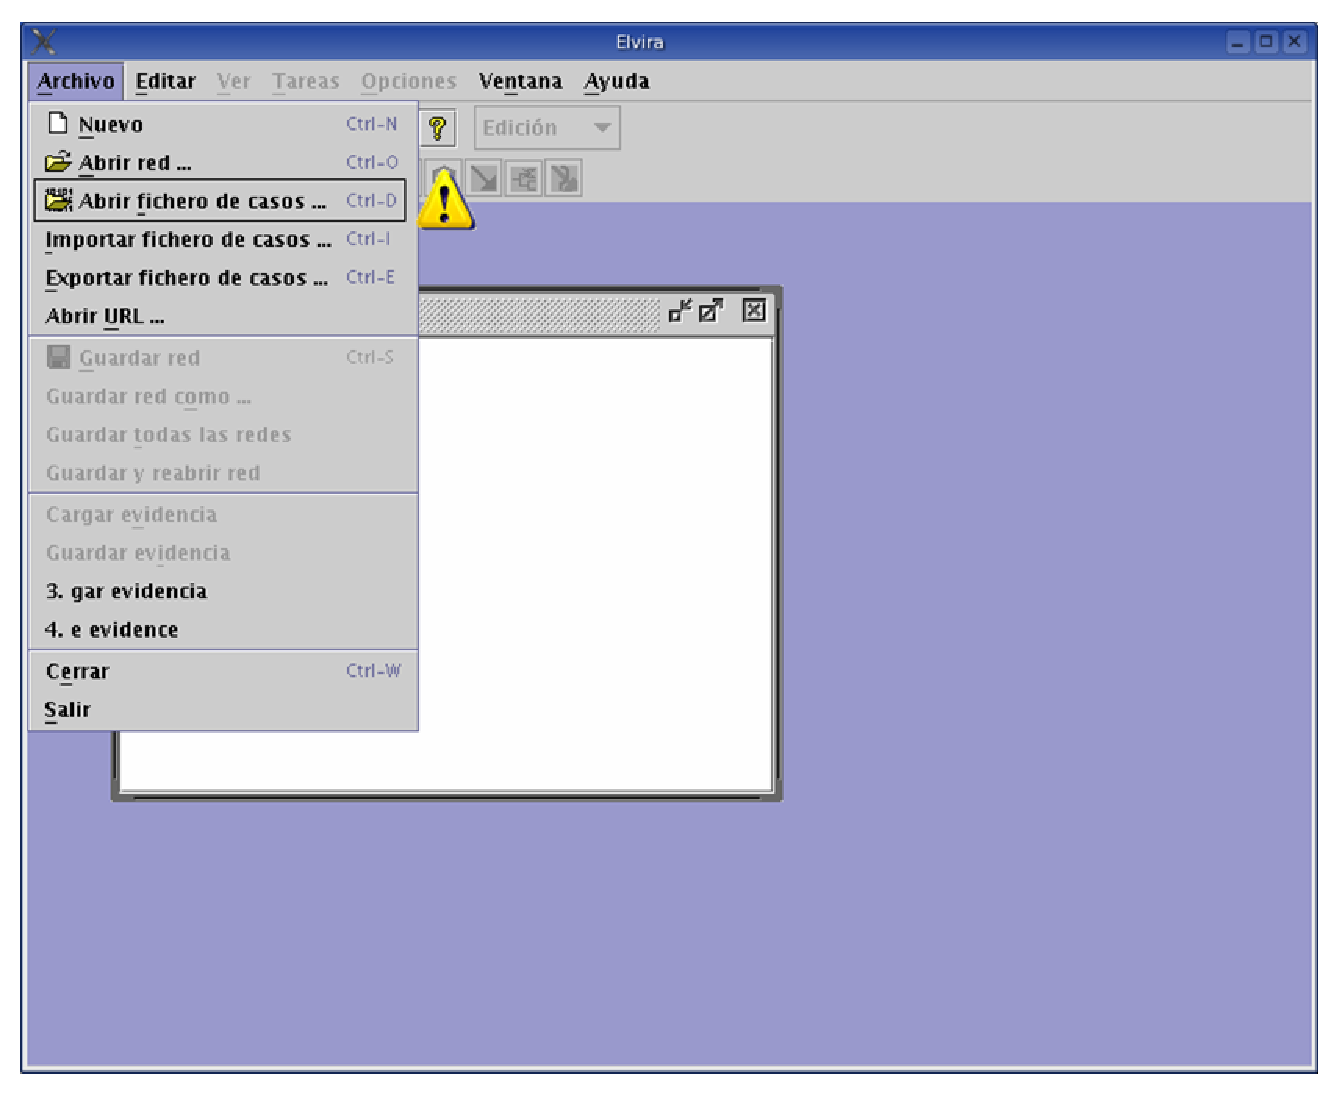
\includegraphics[width=150mm]{Learning/Preprocessing/fig/figure-8.06.ps} 
\caption{Database file loading}
\end{center}
\end{figure}

Then, we will follow the next sequence:
\begin{enumerate}
	\item	Select \verb=Preprocessing Options= in the \verb=Preprocessing Window=, in order to
			access all the preprocessing procedures.
	\item	Select discretization folder \verb=Discretization=.
	\item	Click the \verb=Input Database File= button to select the file that contains the database
			to discretize.
	\item	Click the \verb=Output Database File= to select the discretized database file.
	\item	This is the most critical step, as we must choose between a \verb=MASSIVE=
			or a \verb=NORMAL=, the most normal being \verb=MASSIVE=, as it makes a discretization
			over all the variables with the same algorithm and number of intervals.
			\begin{enumerate}
				\item	Select the algorithm.
				\item	Select the number of intervals.
			\end{enumerate}
			In the case we have chosen \verb=NORMAL=, we will carry out the following steps for each variable:
			\begin{enumerate}
				\item	Decide if we discretize the variable or not.
				\item	Select the algorithm.
				\item	Select the number of intervals.
			\end{enumerate}
	\item	Click the \verb=Process= button.
\end{enumerate}

In figure 8.7 we see the complete process.

\begin{figure}[htb]
\begin{center}
\label{cap08:07}
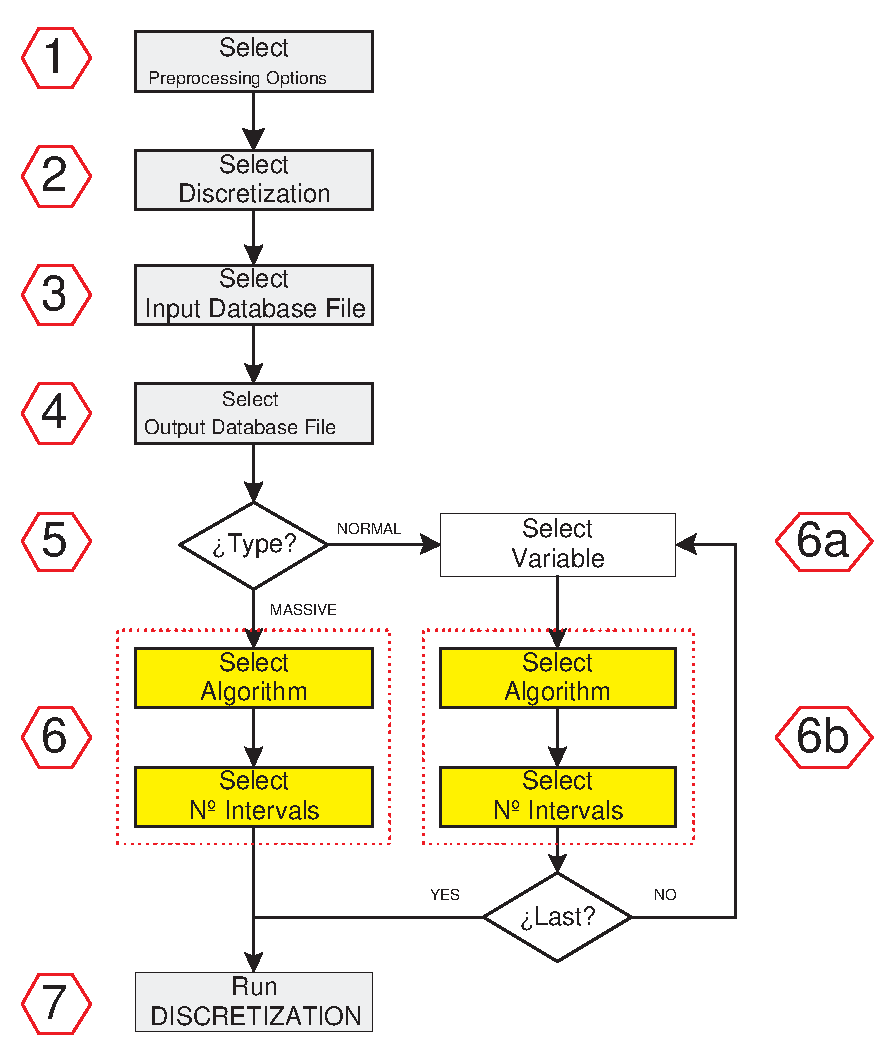
\includegraphics[width=100mm]{Learning/Preprocessing/fig/figure-8.07.ps} 
\caption{GUI: Steps to discretize}
\end{center}
\end{figure}

As we can see, the discretization can be applied over databases of different types. If we have chosen
\verb=NORMAL=, it allows us to decide for each variable if we discretize it or not, the number of intervals,
type of algorithm, \ldots In some cases, this can be specially useful if some variables can not be discretized
in more intervals than a previously fixed one.

The correspondence of this algorithm with the graphical interface can be observed in figure 8.8, but take into
account that the points \verb=6a= and \verb=6b= have not been marked for clarity purposes. In this figure, once
the discretization is executed, we will see a progress bar that will indicate the time spent and when 
the discretization is finished .When it finishes, a dialog box indicating so will appear.

\begin{figure}[htb]
\begin{center}
\label{cap08:08}
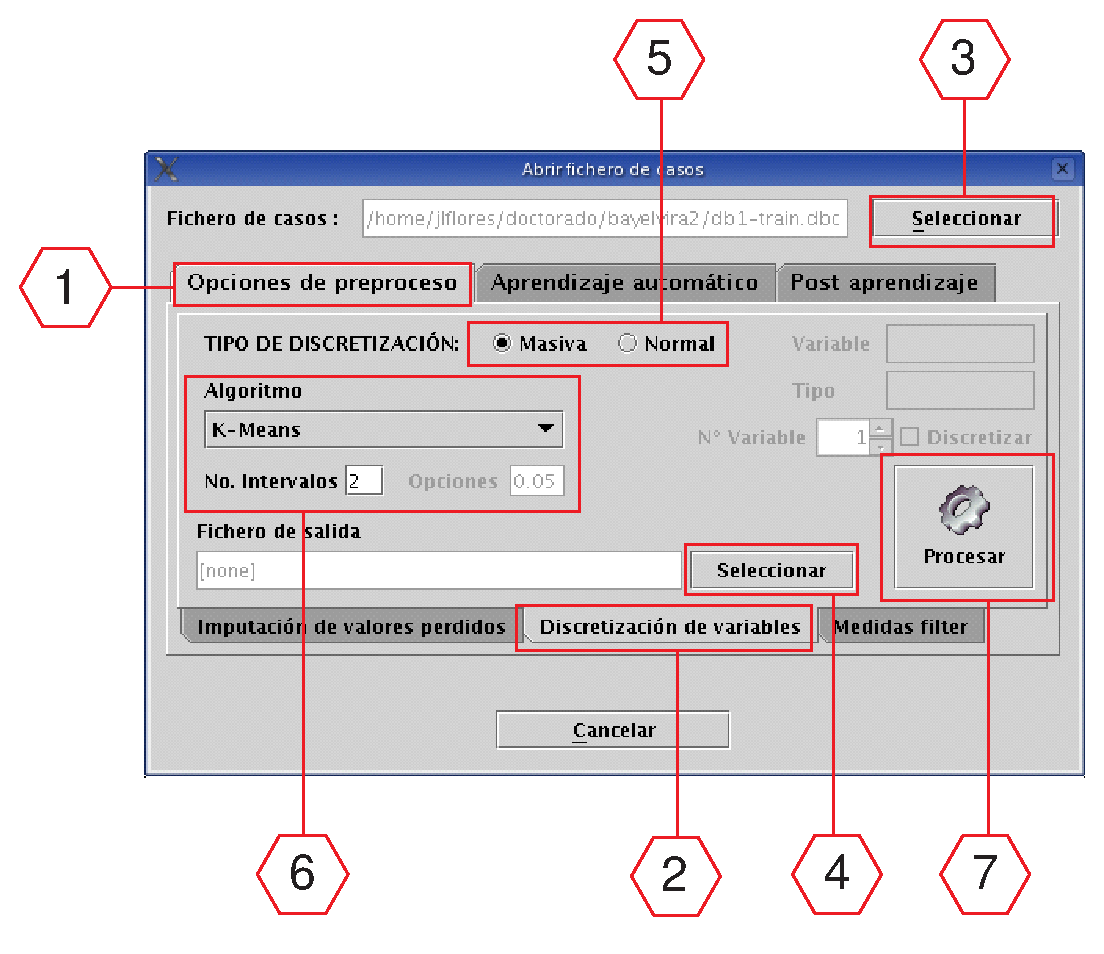
\includegraphics[width=100mm]{Learning/Preprocessing/fig/figure-8.08.ps} 
\caption{GUI Steps}
\end{center}
\end{figure}